\documentclass[a4paper,twoside]{iiththesis}

\usepackage{graphicx}
\book{Thesis}
\title{Machine learning for Compiler}
\degree{Master of Technology}
\department{Computer Science and Engineering}
\submitted{June 2021}
\author{Rohit Aggarwal}
\adviser{--------------}
\addradviser{Dept. of Chem Eng \\ IITH}
\chair{---------}
\addrchair{Dept. of Mech Eng \\ IITH}
\external{----------}
\addrexternal{Dept. of Chem Eng \\ IITM}
\internal{----------}
\addrinternal{Dept. Math \\ IITH}
\coguide{----------}
\addrcoguide{Dept. of Chem Eng \\ IITH}
\abstract{
This is not a  document on how to use latex. It rather explains how to use iiththesis.cls file to write your
thesis for PhD/M.Tech/MSc. This file is generated using the class iiththesis.cls. This document draws a broad picture of the structure and formatting of your thesis. 
}
\acknowledgements{.}
\dedication{.}


\renewcommand{\bibname}{References}
\begin{document}

\chapter{Introduction}
%         The multiple domains are using Machine Learning for achieving the task which was previously very hard, or the result was not that efficient. There are many types of machine learning algorithms for different kinds of functions.

% 	    Every ML algorithms have it’s own usage and are divided into supervised learning, unsupervised learning, semi-supervised learning, and many more. The supervised learning problems are either classification or Regression. The classification is the task in which the model predicts the tag or label from the given labels for a given data point. Tagging the image and sentiment analysis are examples of the classification. In regression, the model predicts the value between an interval. Price of the house, Pollution growth-decline prediction are famous examples for regression.
	
% 	    Deep learning is a type of machine learning in which we use a neural network as the function approximator. The neural networks are some kind of multi-layered perceptrons(MLP). Most of the current works are using Deep learning to achieve state of art. The ImageNet challenge in which major breakthroughs were presented by AlexNet in which they won it with a margin of 15%. Since then, a lot of work has been done.
	
% 	    Similarly, there are works that are done on program representations and code optimization. Some classic works like program tagging, summarization, vulnerability detection, and others. On the code optimization side, device mapping in which code generated in such a way so that it can run efficiently on either of it.
	   
% 	    We have worked on the program representation for LLVM IR. Here, we can generate the Instruction level, function level, and program level embedding. These embedding can be used in many software engineering and optimization tasks depending on the design. We have written a program classification model in TensorFlow and PyTorch for the unseen algorithms. In the coming chapter, we will describe them in detail.	
    	
%     	We have recreated the experimentation of Thread Coeresing Factor which IR2Vec and able to have improved on the state-of-the-art results. It is a compiler optimization task that depends on machine architecture. 

% \chapter{Applying IR2Vec to thread coarsening}
% \section{Introduction to IR2Vec}

% \section{Thread Coarsening Task}
% Thread coarsening~\cite{Volkov-Demmel-10.5555/1413370.1413402} is the process of increasing the work done by a single thread by fusing two or more concurrent threads. Thread coarsening factor corresponds to the number of threads that can be fused together. Selection of an optimal thread coarsening factor can lead to significant improvements~\cite{Magni-SC13-DBLP:conf/sc/MagniDO13} in the speedups on GPU devices and a naive coarsening would lead to a substantial slowdown.

% A thread coarsening factor of a kernel that gives the best speedup on a GPU could give the worst performance with the same coarsening factor on another device (either within or across vendors) because of the architectural characteristics of the device~\cite{magni2014automatic, Stawinoga-10.1145/3194242}. For example, \texttt{nbody} kernel, which has a higher degree of Instruction Level Parallelism, can be better exploited by VLIW based AMD Radeon than SIMD based AMD Tahiti~\cite{magni2014automatic}.

% \subsubsection*{Dataset} 
% In this experiment, we follow the experimental setup proposed by Magni et al.~\cite{magni2014automatic} to predict the optimal thread coarsening factor---among $\{1,2,4,8,16,32\}$---for a given kernel specific to a GPU device. Even for this experiment, we use the dataset provided by Ben-Nun et al.~\cite{ncc}. It consists of about 68 datapoints from 17 OpenCL kernels on 4 different GPUs -- AMD Radeon 5900, AMD Tahiti 7970, NVIDIA GTX 480 and NVIDIA Tesla K20c.
% These kernels are collectively taken from AMD SDK, NVIDIA SDK and Parboil benchmarks.
% A datapoint consists of the kernel and its runtime corresponding to each thread coarsening factor on a particular GPU device.

% \subsubsection*{Experimental Setup}
% Even for this task, we use gradient boosting classifier instead of LSTMs and RNNs to predict the coarsening factor for the four GPU targets. For this experiment, we set the learning rate as 0.05 with 140 decision stumps with 1 level, as the number of data points in the dataset is very low. We use ten-fold cross-validation for measuring the performance.

% \begin{table}[h]
%   \caption{\% improvement in speedup obtained by Flow-Aware encodings when compared to the other methods}
%   \vspace*{-\baselineskip}
%   \label{tab:predictionSpeedup-tc}    \small
%   \begin{tabular}{p{2.5cm}p{1.9cm}p{1.6cm}p{1.5cm}p{2.2cm}p{1.5cm}}
%     \toprule
%     \textbf{Architecture} & \textbf{Magni et al. \cite{o2013portable-grewe}} & \textbf{DeepTune \cite{cummins2017end2end}} & \textbf{DeepTune-TL \cite{cummins2017end2end}} & \textbf{inst2vec \cite{ncc}}\footnotemark  & \textbf{\irtovec  Symbolic}\\
%     \midrule
%     \textbf{AMD Radeon 5900} & 27.66\% & 5.26\% & 5.26\% & 4.35\% & -- \\
%     \textbf{AMD Tahiti 7970} & 25.41\% & 29.37\% & 36.56\% & 18.17\% & 2.08\% \\
%     \textbf{NVIDIA GTX 480} & 45.31\% & 25.21\% & 18.89\% & 23.89\% & 3.98\%\\
%     \textbf{NVIDIA Tesla K20c} & 52.84\% & 15.41\% & 11.98\% & 11.98\% & 0.18\%\\
% \bottomrule
% \end{tabular}
% \end{table}
% \footnotetext{As per the results given in the NCC paper~\cite{ncc}, inst2vec-imm achieves a (arithmetic) mean of $ 1.28\times$, $ 1.18\times$, $ 1.11\times$ and $1\times$ speedup on AMD Radeon, AMD Tahiti, NVIDIA GTX and NVIDIA Tesla; whereas our \textit{Flow-Aware} encodings achieve a (arithmetic) mean of $ 1.25\times$, $ 1.3\times$, $ 1.26\times$ and $ 1.16\times$ respectively.}

% \textit{Speedups.}
% In Fig.~\ref{fig:tcSpeedup}, we show the speedups achieved by our encodings and earlier works on four different platforms -- AMD Radeon HD 5900, AMD Tahiti 7970, NVIDIA GTX 480 and NVIDIA Tesla K20c. 

% On AMD Radeon, both of our encodings achieve a speedup of $ 1.2\times$ when compared to the state-of-the-art speedup of $ 1.15\times$ and $ 1.14\times$ achieved by inst2vec~\cite{ncc} and DeepTune model with transfer learning (DeepTune-TL)~\cite{cummins2017end2end}.
% In AMD Tahiti, \textit{Flow-Aware} encodings achieve a speedup of $ 1.23\times$; \textit{Symbolic} encoding achieves a speedup of $ 1.2\times$, whereas the earlier works by DeepTune-TL and inst2vec achieve a speedup of $ 0.9\times$ and $ 1.04\times$ respectively. In Tab.~\ref{tab:predictionSpeedup-tc}, we show the percentage improvement of speedup obtained by \textit{Flow-Aware} encodings over other methodologies. From the table, we can infer that \textit{Flow-Aware} gives better results for every architecture when compared to the other methods. 

% % \begin{figure}
% %     \centering
% %     \begin{tabular}{@{}c@{}}
% %         \includegraphics[scale=0.55, width=\textwidth]{figures/TC/radeon.pdf}
% %     \end{tabular}
% %     % \vspace{-5cm}
% %     \begin{tabular}{@{}c@{}}
% %         \includegraphics[scale=0.55, width=\textwidth]{figures/TC/tahiti.pdf}
% %     \end{tabular}
% %     \begin{tabular}{@{}c@{}}
% %         \includegraphics[scale=0.55, width=\textwidth]{figures/TC/gtx.pdf}
% %     \end{tabular}
% %     \begin{tabular}{@{}c@{}}
% %         \includegraphics[scale=0.55, width=\textwidth]{figures/TC/tesla.pdf}
% %     \end{tabular}
% %     \caption{Plot showing the speedups achieved by predicted coarsening factors by various methods}
% %     % \vspace*{-\baselineskip}
% %     \label{fig:tcSpeedup}
% %      \vspace*{-0.4cm}
% % \end{figure}

% % \begin{figure}
% %     \centering
% %     \begin{tabular}{@{}c@{}}
% %         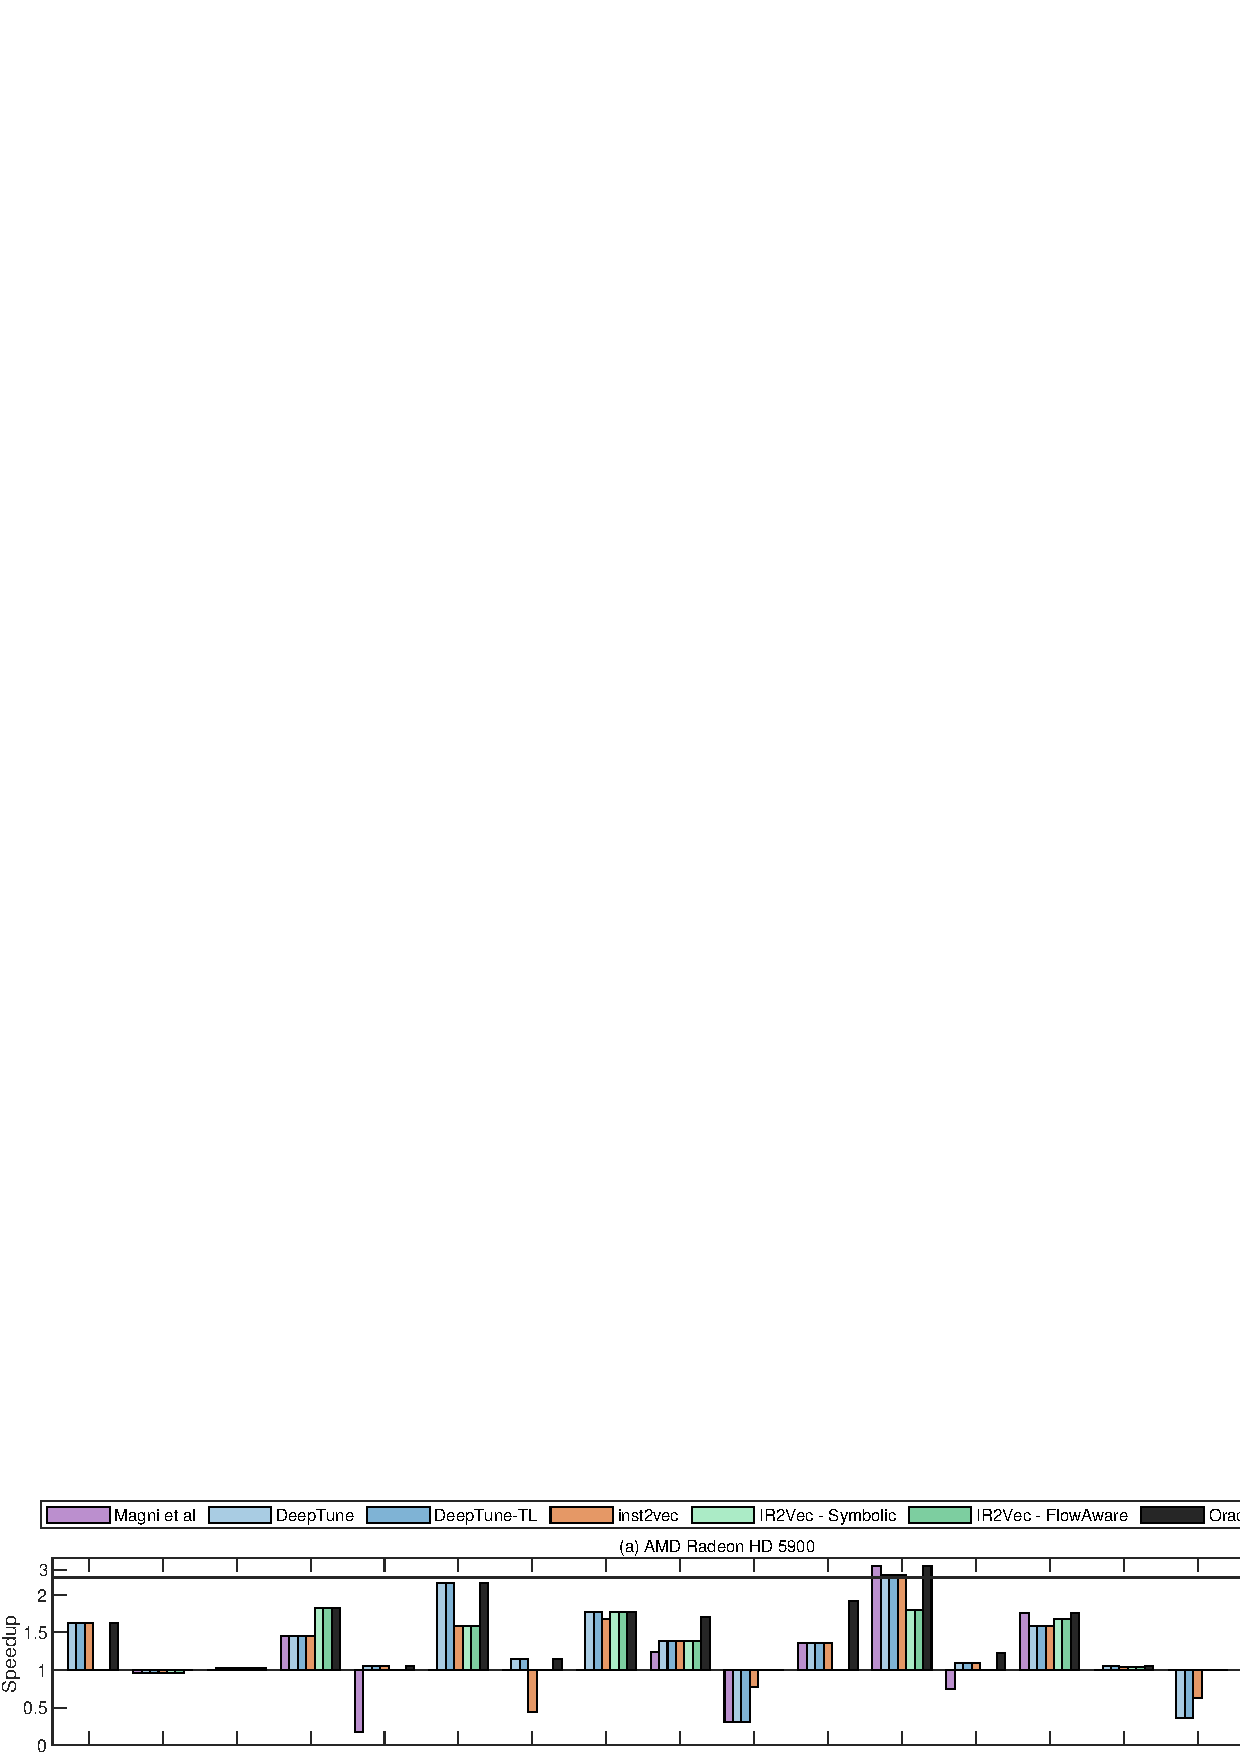
\includegraphics[scale=0.8, width=\textwidth]{figures/TC/new/radeon1-crop.pdf}
% %     \end{tabular}
% %     % \vspace{-5cm}
% %     \begin{tabular}{@{}c@{}}
% %         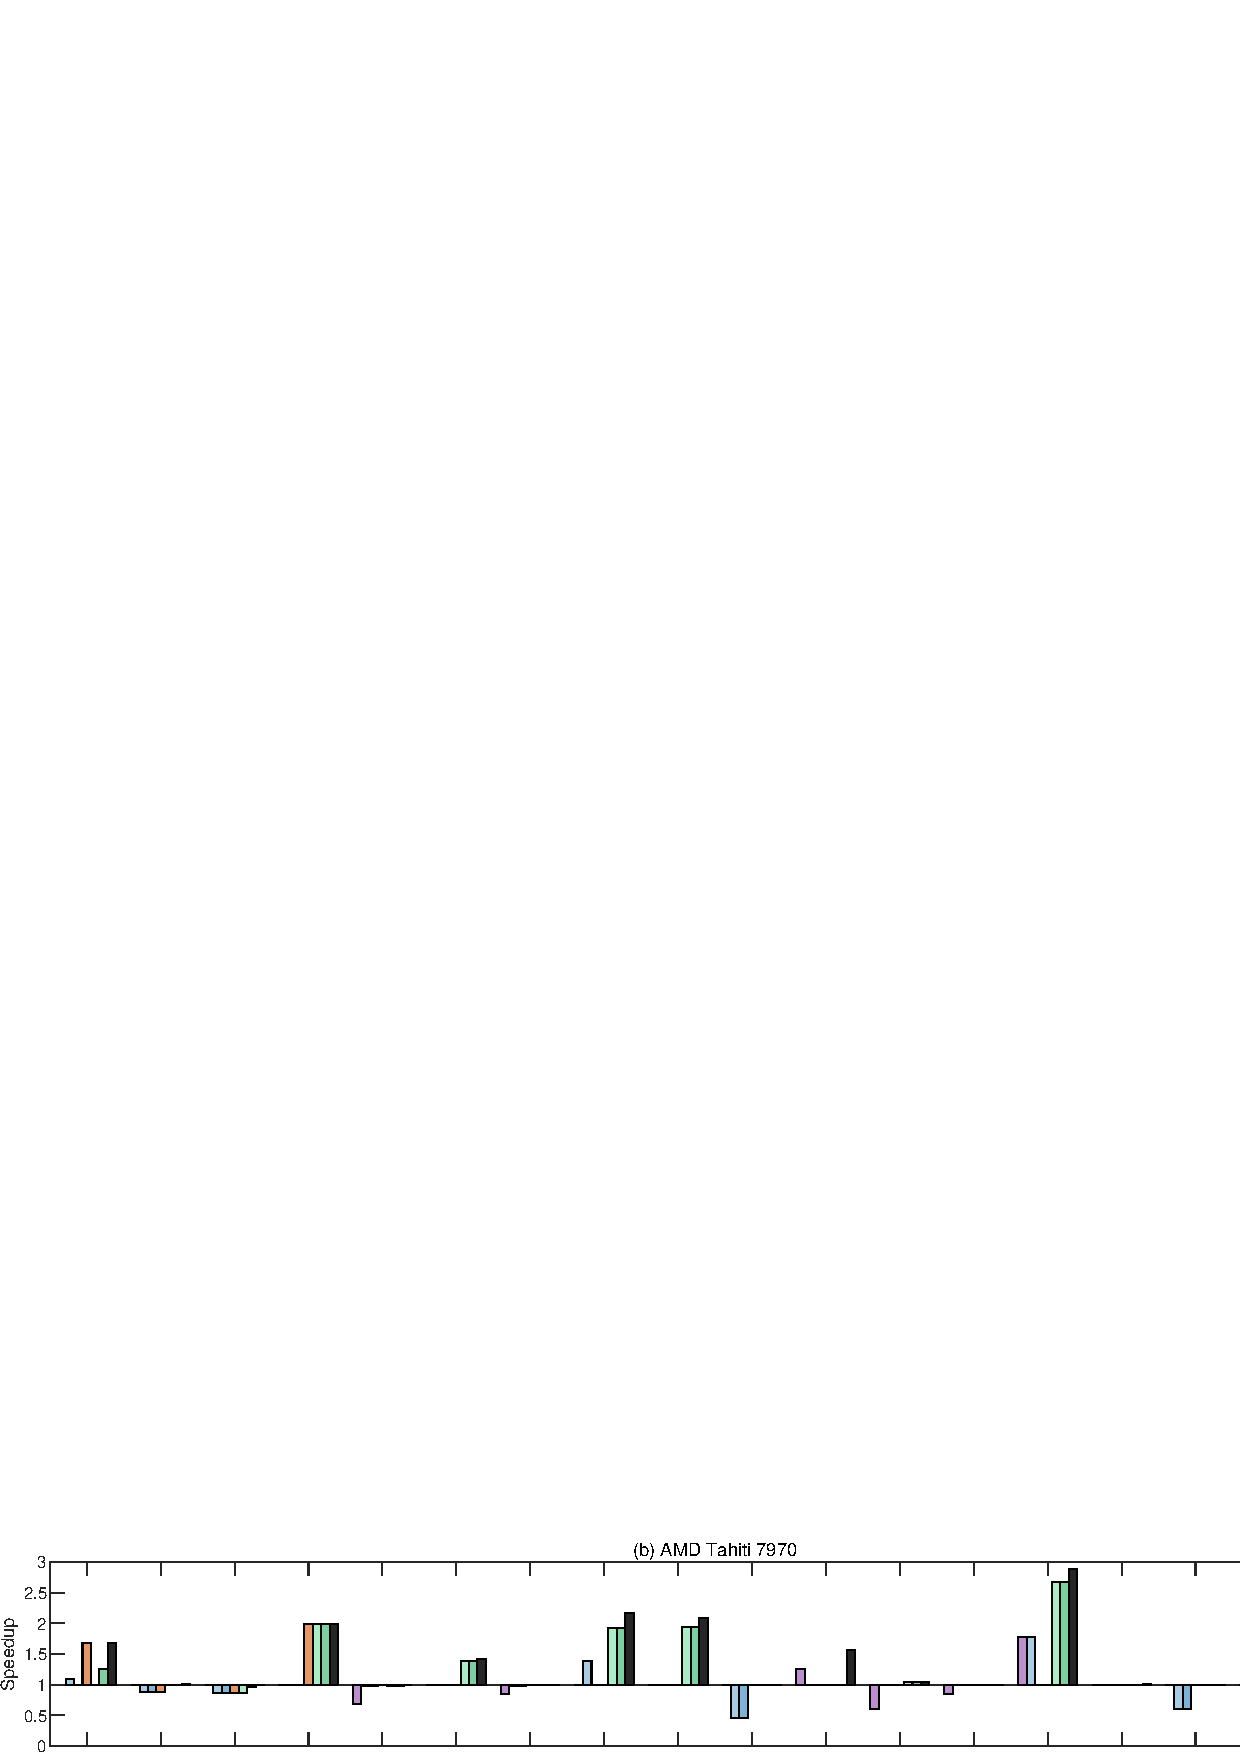
\includegraphics[scale=0.8, width=\textwidth]{figures/TC/new/tahiti2-crop.pdf}
% %     \end{tabular}
% %     \begin{tabular}{@{}c@{}}
% %         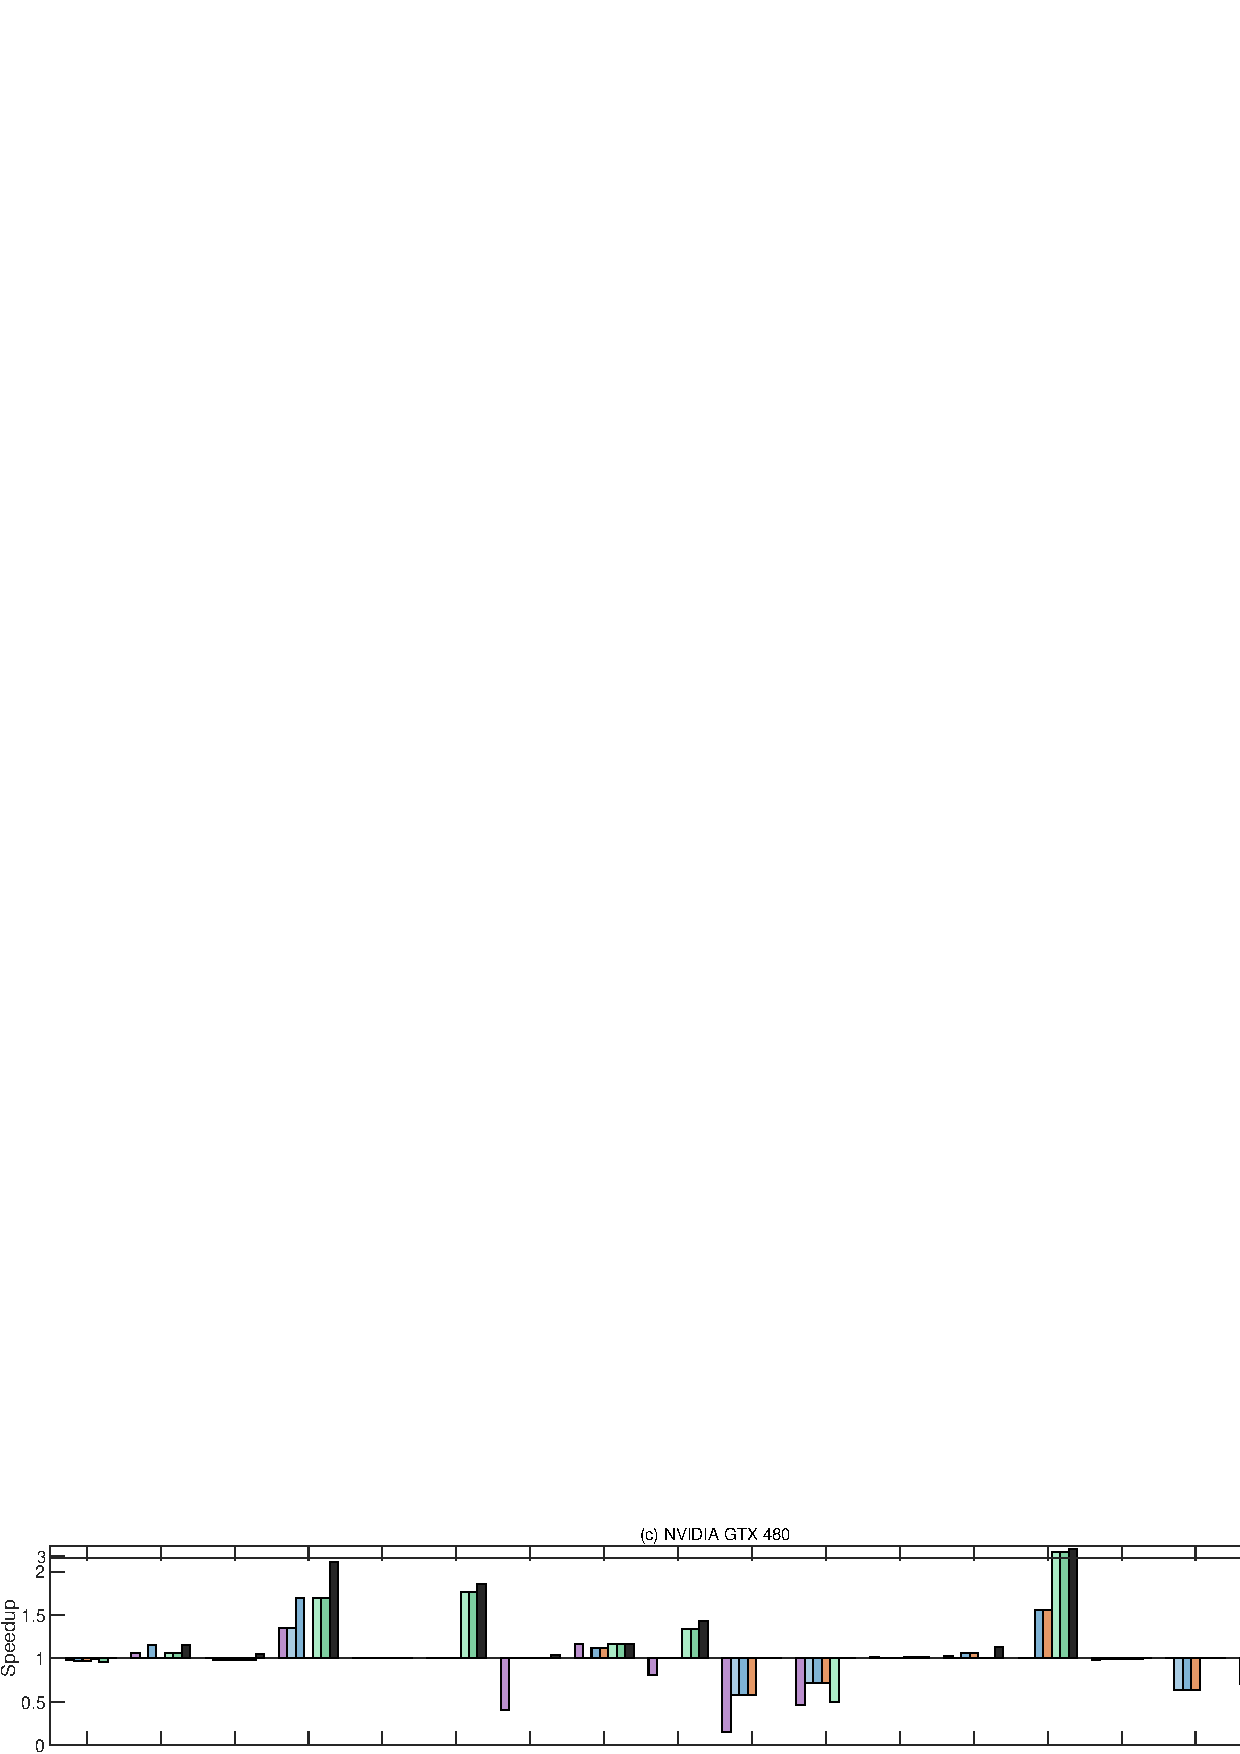
\includegraphics[scale=0.8, width=\textwidth]{figures/TC/new/gtx-crop.pdf}
% %     \end{tabular}
% %     \begin{tabular}{@{}c@{}}
% %         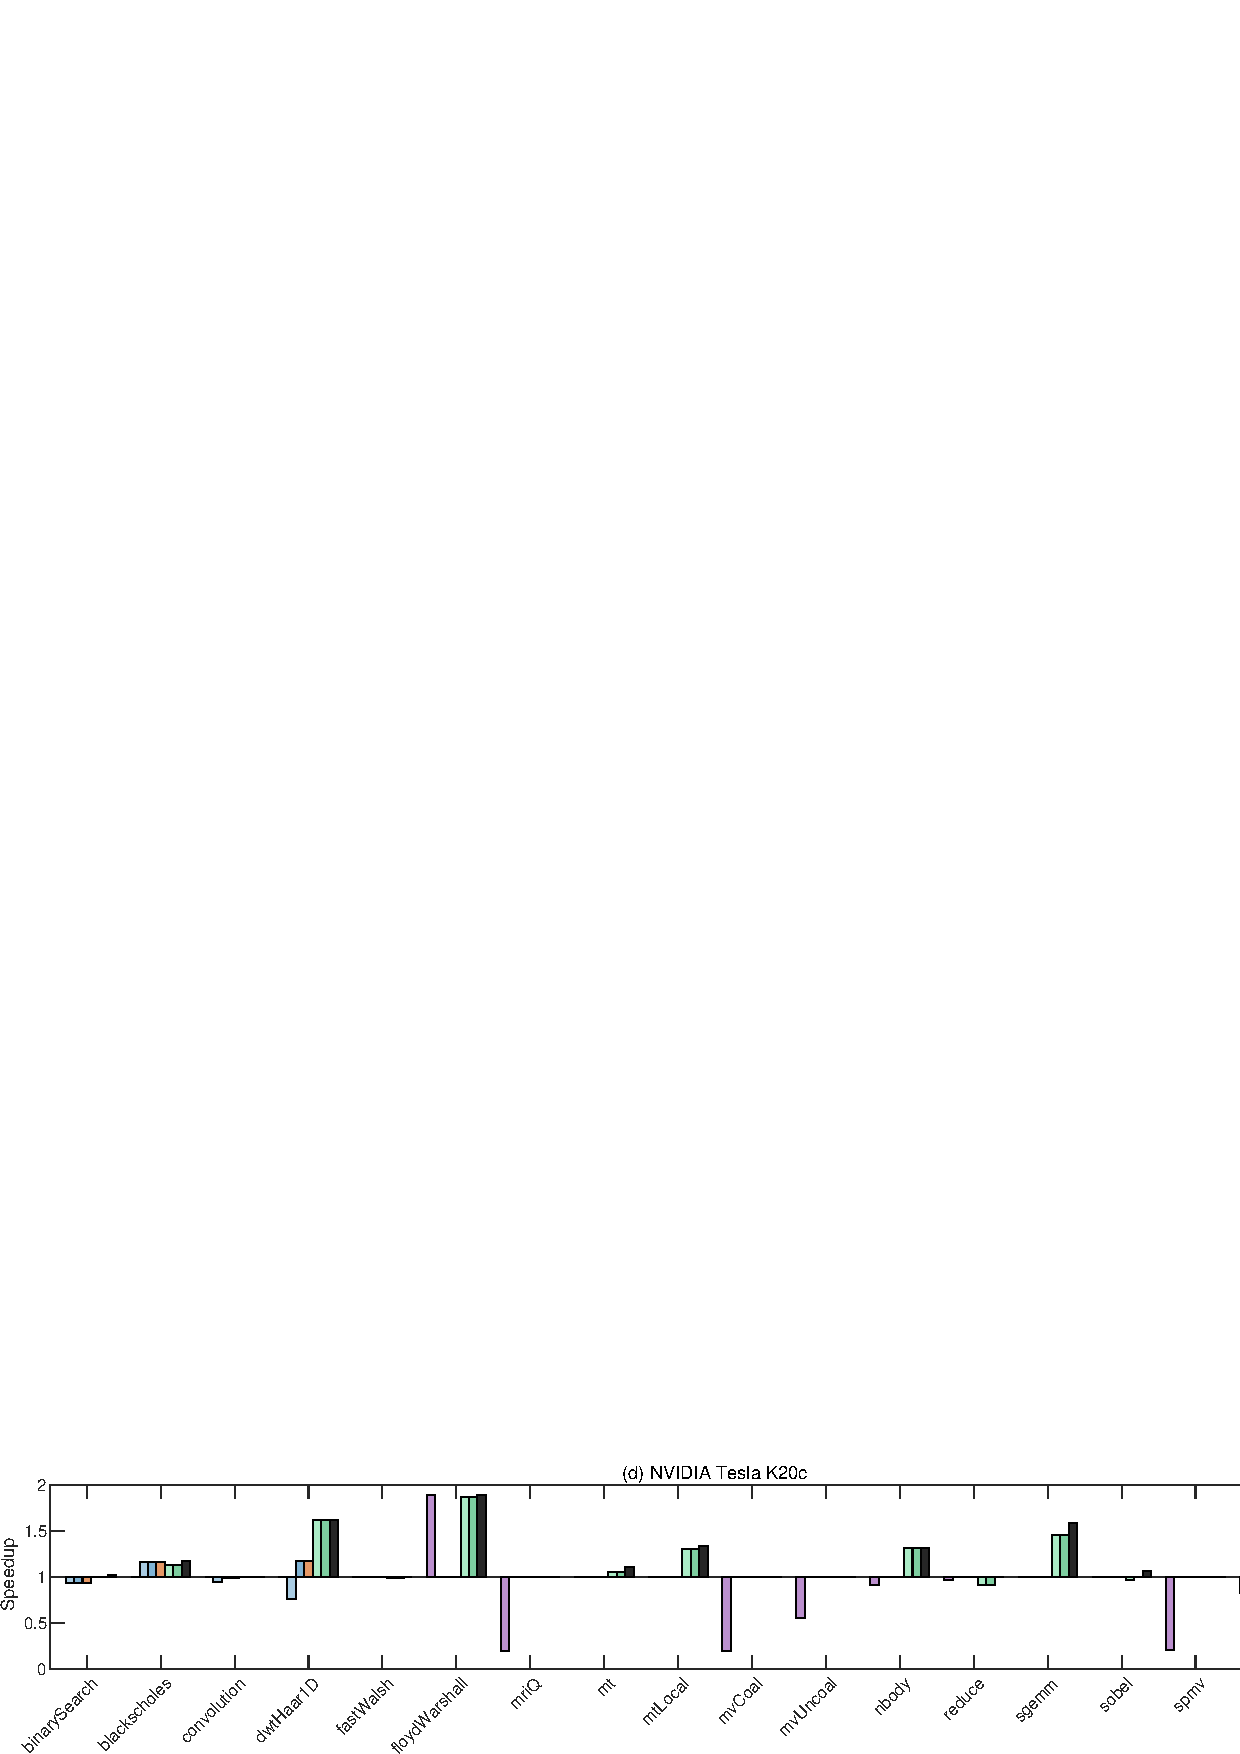
\includegraphics[scale=0.8, width=\textwidth]{figures/TC/new/tesla2-crop.pdf}
% %     \end{tabular}
% %     \caption{Plot showing the speedups achieved by predicted coarsening factors by various methods}
% %     % \vspace*{-\baselineskip}
% %     \label{fig:tcSpeedup}
% %      \vspace*{-0.4cm}
% % \end{figure}

% \begin{figure}
%     \centering
%     \begin{tabular}{@{}c@{}}
%         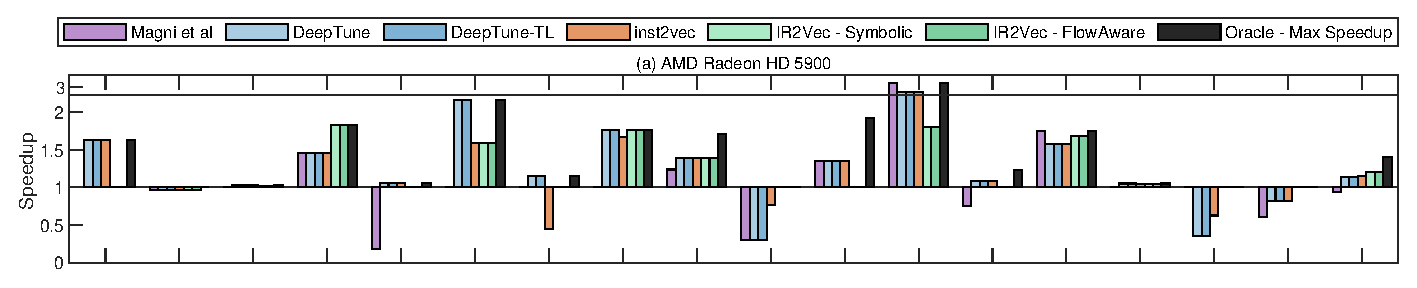
\includegraphics[scale=0.8, width=\textwidth]{figures/TC/new-eps/radeon1-crop.eps}
%     \end{tabular}
%     % \vspace{-5cm}
%     \begin{tabular}{@{}c@{}}
%         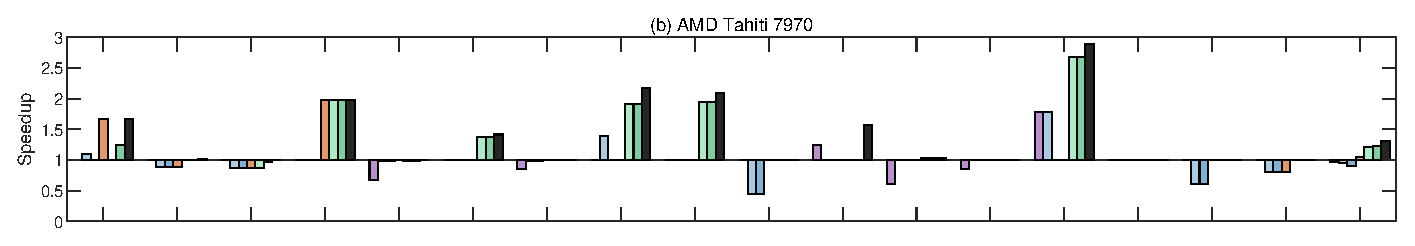
\includegraphics[scale=0.8, width=\textwidth]{figures/TC/new-eps/tahiti2-crop.eps}
%     \end{tabular}
%     \begin{tabular}{@{}c@{}}
%         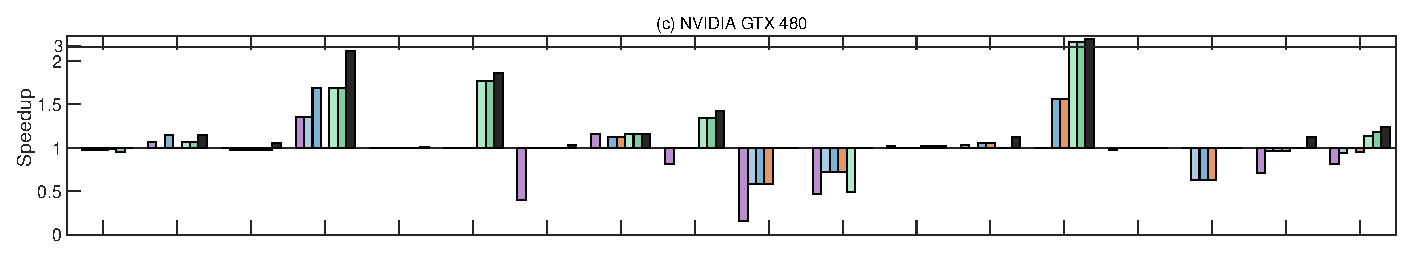
\includegraphics[scale=0.8, width=\textwidth]{figures/TC/new-eps/gtx-crop.eps}
%     \end{tabular}
%     \begin{tabular}{@{}c@{}}
%         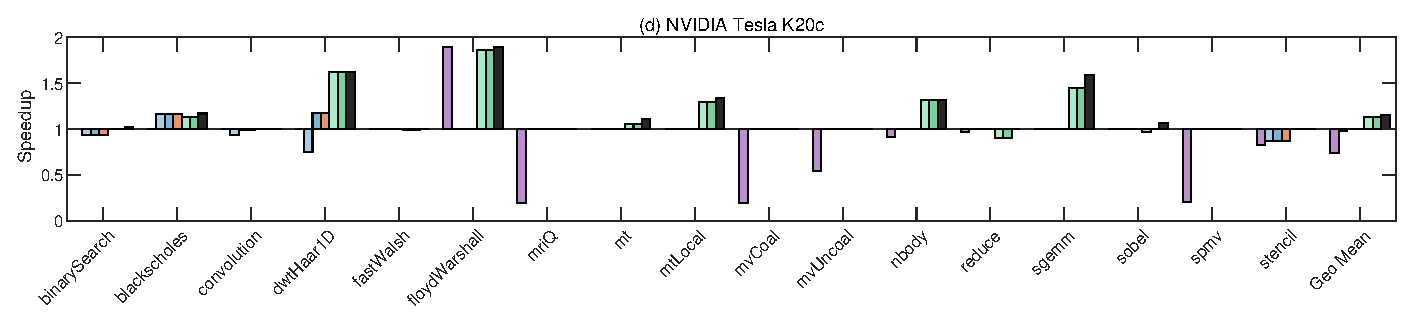
\includegraphics[scale=0.8, width=\textwidth]{figures/TC/new-eps/tesla2-crop.eps}
%     \end{tabular}
%     \caption{Plot showing the speedups achieved by predicted coarsening factors by various methods}
%     % \vspace*{-\baselineskip}
%     \label{fig:tcSpeedup}
%      \vspace*{-0.4cm}
% \end{figure}


% We are the \textit{first ones} to achieve a positive speedup on NVIDIA GTX 480; our \textit{Flow-Aware} and \textit{Symbolic} encodings obtain a speedup of $ 1.18\times$ and $ 1.13\times$ respectively when compared to $ 0.95\times$ and $ 0.99\times$ speedup achieved by inst2vec and DeepTune-TL. 
% We get a speedup of $ 1.13\times$ with both of our proposed encodings on NVIDIA Tesla K20c. In contrast, DeepTune-TL and inst2vec obtain a speedup of $ 1.01\times$ on this platform.

% On average, it can be seen that both encodings outperform the earlier methods for prediction of the thread coarsening factor on all the four platforms under consideration. 

% \textit{Slowdown.}  Magni et al.~\cite{magni2014automatic} observe that \texttt{spmv} and \texttt{mvCoal} kernels have irregular dependences that causes a poor response to coarsening, and hence no performance improvement for them is possible.
% For these kernels, \irtovec obtains the baseline speedup \textit{without} resulting in a slowdown. In contrast, the earlier models result in negative speedups (Deeptune results in a slowdown upto $0.36$ $\times$ in AMD Radeon and inst2vec results in a slowdown of upto $0.63$ $\times$ in AMD Radeon and NVIDIA GTX). 
% The same argument applies for \texttt{stencil} kernel (an iterative Jacobi stencil on 3D-grid), where the coarsening leads to slowdown (except in NVIDIA GTX), while \irtovec still obtain the baseline speedup.

% When compared to the other methods, we obtain the best speedup on about 70\% of the kernels on all platforms. 
% It can be observed that the \textit{Flow-Aware} encodings \textit{rarely lead to slowdowns}; this happens in only 8/68 cases (17 benchmark-suits, across 4 platforms), even on these eight cases, the speedup is still close---within 10\%---of the baseline. 
% Whereas, predictions by inst2vec and DeepTune-TL result in a slowdown in 18 and 21 cases.
% We believe that this is because of the flow information associated with the obtained vectors.

% \chapter{Supervised Learning}
% \section{Introduction}
% Supervised Learning is the field of machine learning in which the model is trained against known label or tags. The model for a given data point can't predict any thing not mentioned in the vocabulary. There are some fixit numbers of label for a machine learning task.

% \section{Background}
% In case of the image classification, there is a image dataset and each image is labeled. We run the training using the given images as the input and predict the image label. Given the true value and predicted value, we calculate the loss with is used to generate gradient.

% \section{Methodology}
% On the similarly ground, We are trying to do algorithm recognition. Here given the bunch of the program, we want to predict to give algorithm class the program belong to.

% We developed an classifier in TensorFlow which can classify the program respectively. 
% \subsection{DataSet}
% We have selected the POJ-104 dataset\ref{} for our experiments. It has 104 type of different program which acts like class or label and each class has approximately ~500 programs. We have splitted this dataset into 3:1:1(training:testing:validation).

% \subsection{Embedding Generation}
% I have used IR2Vec to generate the embedding for the programs. For each program, we get a 300 dimension vector and it's corresponding label.

% \subsection{Model Architecture}
% The first input layer expects a 300-dimension vector which is followed by simple three layered Multi-Level Precptron(MLP) with a softmax layer for output. The Categorical cross entropy Loss is used as the loss function and Adam as the optimizer. The whole training run for 100 epochs.

\section{Results}

% Table~\ref{tab-acc} rather than table~\ref{tab-acc}.
\begin{table}[h]


\begin{tabular}{l l l l}
\hline
Percentage & TBCNN & inst2vec &  Ours\\
\hline
Accuracy(\%) & 94 & 94.83 & 96.2 \\
\hline
\end{tabular}
\centering
\caption{Compare the accuracy percentage.}
\label{tab-acc}
\end{table}

\begin{verbatim}
\documentclass{iiththesis}
\end{verbatim}
The student need not to worry about the structure of the front matter. The class file takes the following information to generate the front matter
% \begin{itemize}
% \item Title
% \item Degree
% \item Book
% \item Department
% \item Submission date
% \item Author
% \item Chairman (optional)
% \item External examiner (optional)
% \item Internal examiner  (optional)
% \item Adviser
% \item Co-adviser (optional)
% \item Acknowledgment (optional)
% \item Dedication (optional)

% \end{itemize}
\subsection{Title}
$ \backslash $title\{tile of the thesis\} will generate the tile of your thesis.

\subsection{Degree}
Use $ \backslash $degree\{Master of Technology\} to input your degree.

\subsection{Book}
Use $ \backslash $book\{\} to input nature of report. For PhD ``Dissertation" is recommended and
for M.Tech ``Thesis" is recommended.

\subsection{Department}
Use $ \backslash $department\{Your department\} to input your department name.

\subsection{Submission date}
Use $ \backslash $submitted\{June 2011\} to input date of submission.


\subsection{Author}
Use $ \backslash $author\{Student name\} to input the author name.

\subsection{Committee members}
The committee members consists of chairman, adviser, and examiners.  Use the following commands to include the committee members
\begin{itemize}
\item $ \backslash $adviser\{Your adviser\}
\item $ \backslash $chair\{Committee chairman\}
\item $ \backslash $external\{External examiner \}
\item $ \backslash $internal\{Internal examiner \}
\item $ \backslash $coguide\{Co-Adviser\}

\end{itemize}

The affiliation of each examiner can be provided using the following environments
\begin{itemize}
\item $ \backslash $addradviser\{Address line 1 $ \backslash \backslash $ Address line 2\}
\item $ \backslash $addrchair\{Address line 1 $ \backslash \backslash $ Address line 2\}
\item $ \backslash $addrexternal\{Address line 1 $ \backslash \backslash $ Address line 2 \}
\item $ \backslash $addrinternal\{Address line 1 $ \backslash \backslash $ Address line 2 \}
\item $ \backslash $addrcoguide\{Address line 1 $ \backslash \backslash $ Address line 2\}

\end{itemize}


\subsection{Acknowledgments}
This is optional. Use the acknowledgment environment $ \backslash $acknowledgments\{\}   to create the acknowledgement.
You may write your acknowledgment in an external file, and that can be incorporated into the main tex file using the $ \backslash $input\{filename\}.


\subsection{Dedication}
This is optional. Use the dedication environment $ \backslash $dedication\{\}   to create the acknowledgement.
You may write your dedication in an external file, and that can be incorporated into the main tex file using the $ \backslash $input\{filename\}.

\section{Where to put the above environments}
All the above mentioned environments must be defined before starting the document. i.e. before the environment
 $ \backslash $begin\{document\}.

\chapter{Citation}
\section{Single citation}
The cite command can be used to create any reference~\cite{Achenbach1995}. i.e. 
\begin{verbatim}
\cite{bibtex_key}
\end{verbatim}


\section{Multiple citation}
You can also cite multiple references using the cite option~\cite{Achenbach1995,Aguiar2004}.. i.e
\begin{verbatim}
\cite{bibtex_key1, bibtex_key2}
\end{verbatim}

Books and Thesis may be cited in the same way~\cite{Bard2001,Iordanidis2002}. The student need not to worry about difference in citation style for journal article, conference, books, thesis etc. This is taken care by bibliography style-file iiththesis.bbl. You are strongly recommended to use $ \backslash $ bibliography{•} rather than individual bibtex entries. By using $ \backslash $bibliography{•} you will never have references which are not cited in the text. You can use any reference manager to create your collection of bibliography.bib. For instance JabRef and Mendeley are reference managers which are freely available.

\chapter{Figures}
\section{Referencing figures}
The figure where ever possible must be centered. Each figure must have a caption centered to the figure. Every single figure in the document must be referred in the text. For example IITH logo is displayed in Fig.~\ref{iithlogo}.

\begin{figure}[h]
\centering
\includegraphics[scale=0.5]{logo}
\caption{This is IITH logo}
\label{iithlogo}
\end{figure}

Use ``Fig". to refer to a figure if the reference to it appears not at the beginning of a sentence. If the sentence starts with reference to figure use ``Figure". For instance refer to the following text.
Figure~\ref{iithlogo} is a compressed logo of IITH.\\

\section{File formats}
You can use jpeg, png, pdf, or eps file format for the figures. However, depending on the file type you will have to use either \textit{pdflatex} or \textit{latex}. Please refer to Chp.~\ref{compiling} for further details.


\chapter{Tables}

\section{Referencing tables}
The tables where ever possible must be centered. The table caption must appear at the top of the table and must be centered to the table. Every table in the document must be referred in the text. Please use capitalized ``T" whenever a reference to table is made. i.e Table~\ref{extable} rather than table~\ref{extable}.
\begin{table}[h]
\centering
\caption{This is an example table.}
\begin{tabular}{l l}
\hline
Parameter & Value \\
\hline
Density & 1 \\
Specific heat & 1 \\
\hline
\end{tabular}
\label{extable}
\end{table}

\chapter{Compiling the \textit{.tex} file }
\label{compiling}

\section{Options}
If you are using jpeg or pdf format for the figures please use\textit{pdflatex} to compile the tex file. If you are using eps format you can use \textit{latex} command to compile the tex file. The \textit{latex} command will create \textit{dvi} output which may be converted to \textit{pdf} by using \textit{dvipdf} on any linux distribution. 

\section{Compilation sequence}
You have to execute the following sequence to commands to get the proper output file.
\begin{verbatim}
latex thesis.tex
bibtex thesis
latex thesis.tex
latex thesis.tex
\end{verbatim}
Notice that you have to tex the document twice after running bibtex.\\

\clearpage
\newpage
\addcontentsline{toc}{chapter}{References} % Please do not remove this
\bibliographystyle{iiththesis}
\bibliography{references}
\end{document}
